% =====================================================================
%  The Foreign Exchange Rate  --  Member 1 sections (draft for merge)
%  Introduction to Economics, Monsoon 2026
%  Compile with XeLaTeX (latexmkrc selects it automatically on Overleaf)
% =====================================================================
\documentclass[11pt]{article}
\usepackage{fxstyle}
\usepackage{xurl}

\begin{document}

\chaptertitle{Introduction to Economics \textperiodcentered{} Teaching chapter}
             {The Foreign Exchange Rate}
             {What is the rupee worth, and why does it keep changing?}

% ============================================================
%  INTRODUCTION: Meera's dollar problem        (Member 1)
%  Main-text words: see word count in README (boxes excluded)
% ============================================================
\section*{Introduction: Meera's dollar problem}
\addcontentsline{toc}{section}{Introduction}

In October 2026, Meera, a Class 12 student in Chennai, got the email her family had been waiting for: a college in the United States had offered her a place. The first-year fees were US\$40,000, exactly what the college had charged a year earlier. Yet when her father asked his bank what the fees would cost in rupees, the answer was about ₹2.5 lakh more than it would have been a year before.\sidenote{The fees are hypothetical. The exchange rates are real closing rates: ₹88.67 per US dollar on 13 October 2025 (Business Standard, 2025) and ₹95.05 on 15 October 2026 (HDFC Sky, 2026). 40,000 × (95.05 − 88.67) = ₹2,55,200.} The college had not raised its price. The price of the dollar had gone up.

Meera's uncle Ravi, an electrician in Dubai, had the opposite surprise. Every month he sends part of his salary home to his parents in Thanjavur. This year the same amount arrived as more rupees than before.

One family, one price, and two very different outcomes. This chapter explains what that price is, who sets it, and why it keeps moving.

\begin{keypoints}{Questions this chapter answers}
\begin{itemize}
  \item Why does one country's money have a price in another country's money?
  \item Who buys and sells currencies, and why?
  \item What decides that price, and why does it change so often?
  \item How do countries, and the Reserve Bank of India, manage their exchange rates?
  \item Who gains and who loses when the rupee rises or falls?
\end{itemize}
\end{keypoints}

% ============================================================
%  SECTION 1: What is an exchange rate?          (Member 1)
% ============================================================
\section{What is an exchange rate?}

Chai in Chennai is paid for in rupees, but coffee in New York needs US dollars and a meal in Dubai needs dirhams. So whenever goods, services or savings cross a border, one currency has to be swapped for another. The price of that swap is the \keyterm{exchange rate}{The price of one currency in terms of another, for example ₹95 per US dollar.}: the price of one currency in terms of another (National Council of Educational Research and Training [NCERT], 2007). In India it is set mainly by buyers and sellers in a market, and like the price of onions it can change from minute to minute.

Indian banks write the rate as a \keyterm{direct quote}{The price of one unit of foreign currency in home currency, e.g.\ US\$1 = ₹95.}, ``US\$1 = ₹95'', which is the number of rupees needed to buy one dollar (Jayadev, 2021). Flip it and you get the \keyterm{indirect quote}{How much foreign currency one unit of home currency buys, e.g.\ ₹1 = US\$0.0105.}, ``₹1 = US\$0.0105'', which is the number of dollars one rupee buys. This chapter always uses the direct quote, rupees per dollar (₹/\$), so a bigger number means a weaker rupee. At ₹95 instead of ₹88, every rupee buys fewer dollars \seesec{Appreciation and depreciation: who wins, who loses?}.

\begin{figure}[htbp]
  \centering
  \begin{minipage}[c]{0.40\linewidth}
    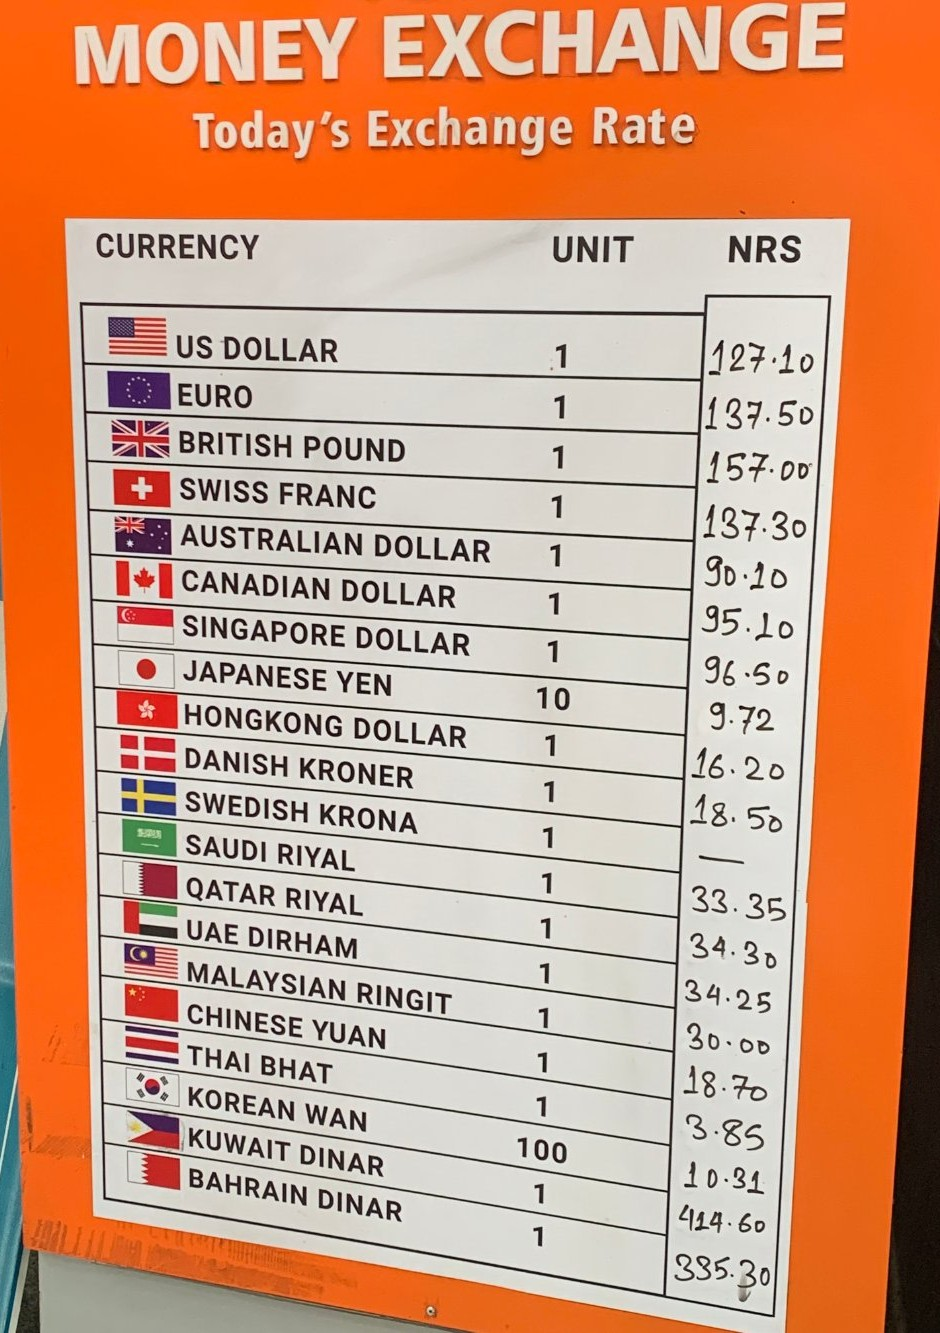
\includegraphics[width=\linewidth]{images/kathmandu_board.jpg}
  \end{minipage}\hfill
  \begin{minipage}[c]{0.56\linewidth}
    \caption{A money exchange board at Kathmandu airport, January 2023.}
    \label{fig:m1-board}
    \small\sffamily
    Each row is a \emph{direct quote}: the price of one unit of a foreign currency in Nepalese rupees (NRs). A US dollar costs NRs~127.10 and a UAE dirham, the currency Ravi earns, about NRs~34. The Japanese yen is priced per 10 yen, because a single yen is worth very little.
    \figsource{Photograph by Chainwit. (2023), \href{https://commons.wikimedia.org/wiki/File:Arrival_at_Kathmandu_Tribhuvan_Airport_(01-2023)_-_img_06.jpg}{Wikimedia Commons}, \href{https://creativecommons.org/licenses/by/4.0/}{CC BY 4.0}, cropped.}
  \end{minipage}
\end{figure}

\begin{didyouknow}{Every board hides two prices}
Banks and money changers quote two rates for each currency: a lower rate at which they buy it from you and a higher rate at which they sell it to you. Suppose a bank buys dollars at ₹93.50 and sells them at ₹96.50. Change ₹10,000 into dollars and you get US\$103.63. Change them straight back and you get only ₹9,689. The missing ₹311 is the bank's earning, called the \textbf{spread}. Spreads are usually widest for cash at airport counters, which is why travellers lose the most there.
\figsource{The rates in this example are hypothetical.}
\end{didyouknow}

\subsection{Why everyone watches the dollar}
Why does the news talk only about the rupee's price in dollars? Because the dollar is the world's working currency. In April 2025 it was on one side of 89 per cent of all currency trades (Bank for International Settlements [BIS], 2025). Crude oil, India's biggest import, is priced in dollars, and only about 6 per cent of India's exports are invoiced in rupees (Reserve Bank of India [RBI], 2026a). Since July 2022 the RBI has allowed Indian firms to settle foreign trade in rupees (RBI, 2022), but most still choose the dollar, because almost everyone, everywhere, will accept it.

The dollar even reaches currencies that seem unrelated. The UAE dirham, which Ravi earns, has been fixed at 3.6725 dirhams per US dollar since 1997 (Nagraj, 2024). So when a dollar costs more rupees, so does a dirham, and every dirham Ravi sends home turns into more rupees.

% ============================================================
%  SECTION 2: The foreign exchange market        (Member 1)
% ============================================================
\section{The foreign exchange market: who needs dollars and who supplies them?}

Currencies are bought and sold in the \keyterm{foreign exchange market}{The market in which currencies are traded for one another. Also called the forex market.}, or forex market. It has no building and no closing bell. It is a worldwide network of banks, dealers and large firms that trade with each other electronically, and as the day moves from Tokyo and Singapore to Mumbai, London and New York, the trading moves with it (Greenlaw et al., 2022).

Figure~\ref{fig:m1-flow} sorts the people in this market into two groups. Importers, students and travellers abroad, Indians investing abroad and anyone repaying a foreign loan need dollars. Together they make up the \keyterm{demand for foreign exchange}{The foreign currency that residents want, to pay for imports, study and travel abroad, investment abroad and foreign loans.}. Exporters like Selvi, whose garment unit in Tiruppur sells T-shirts to American shops, workers abroad like Ravi who send home \keyterm{remittances}{Money that people working abroad send home to their families.}, foreign tourists and foreign investors all bring dollars in. They make up the \keyterm{supply of foreign exchange}{The foreign currency flowing into a country from its exports, remittances, tourists and foreign investment.} (NCERT, 2007). Every deal is two purchases at once: when Meera's father buys dollars, he is also selling rupees (Greenlaw et al., 2022). The exchange rate is the price at which the two sides match \seesec{How the exchange rate is determined: demand and supply}.

\begin{figure}[!htb]
  \centering
  \resizebox{\linewidth}{!}{% Figure M1-2: who demands and who supplies US dollars in India's forex market.
% Drawn in TikZ so it stays sharp and editable. Uses colours from fxstyle.sty.
\begin{tikzpicture}[
  font=\sffamily\small, every node/.append style={execute at begin node={\spaceskip=0.24em plus 0.04em minus 0.02em\relax}},
  item/.style={draw=none, fill=white, rounded corners=1.2mm, minimum height=9.2mm,
               text width=48mm, align=left, execute at begin node={\hyphenpenalty=10000\relax}, inner xsep=7pt, inner ysep=3pt},
  head/.style={text=white, font=\sffamily\bfseries, align=center, text width=52mm,
               minimum height=12mm, rounded corners=1.5mm},
  who/.style={font=\sffamily\scriptsize\itshape, text=fxmuted},
  flow/.style={-{Stealth[length=3.2mm,width=2.6mm]}, line width=1.6pt},
]
% ---- left column: demand ----
\node[head, fill=fxorange] (dh) at (0,0)
  {Who wants dollars?\\[-1pt]{\footnotesize\mdseries demand for foreign exchange}};
\node[item, below=3mm of dh] (d1) {\textbf{Importers}\\[-1pt]{\footnotesize crude oil, gold, electronics, machines}};
\node[item, below=2mm of d1] (d2) {\textbf{Students and travellers abroad}\\[-1pt]{\footnotesize \textcolor{fxorange}{e.g.\ Meera's college fees}}};
\node[item, below=2mm of d2] (d3) {\textbf{Indians investing abroad}\\[-1pt]{\footnotesize shares, property, firms}};
\node[item, below=2mm of d3] (d4) {\textbf{Repaying foreign loans}\\[-1pt]{\footnotesize firms and government}};
\begin{scope}[on background layer]
  \node[fill=fxorange!10, rounded corners=2mm, inner sep=3mm, fit=(dh)(d4)] (dbox) {};
\end{scope}

% ---- right column: supply ----
\node[head, fill=fxteal] (sh) at (13.4,0)
  {Who brings dollars in?\\[-1pt]{\footnotesize\mdseries supply of foreign exchange}};
\node[item, below=3mm of sh] (s1) {\textbf{Exporters}\\[-1pt]{\footnotesize \textcolor{fxteal}{e.g.\ Selvi's T-shirts}, IT services}};
\node[item, below=2mm of s1] (s2) {\textbf{Remittances}\\[-1pt]{\footnotesize \textcolor{fxteal}{e.g.\ Ravi's money from Dubai}}};
\node[item, below=2mm of s2] (s3) {\textbf{Foreign tourists in India}\\[-1pt]{\footnotesize hotels, travel, shopping}};
\node[item, below=2mm of s3] (s4) {\textbf{Foreigners investing in India}\\[-1pt]{\footnotesize FDI and FPI}};
\begin{scope}[on background layer]
  \node[fill=fxteal!10, rounded corners=2mm, inner sep=3mm, fit=(sh)(s4)] (sbox) {};
\end{scope}

% ---- centre: the market ----
\coordinate (mid) at ($(dbox.east)!0.5!(sbox.west)$);
\node[fill=fxnavy, text=white, rounded corners=3mm, text width=36mm, align=center,
      minimum height=34mm, inner sep=6pt] (mkt) at (mid)
  {\heavysans\large Foreign\\exchange market\\[5pt]
   {\footnotesize\sffamily banks and other authorised dealers, regulated by the RBI}};
\node[fill=white, draw=fxnavy, line width=0.8pt, rounded corners=1.5mm, below=4mm of mkt,
      align=center, text width=34mm, inner sep=4pt] (price)
  {{\footnotesize\color{fxmuted}the price that clears it}\\[-1pt]{\heavysans\color{fxnavy}\large ₹ per US dollar}};

% ---- flows ----
\draw[flow, fxorange] (dbox.east |- mkt.150) -- (mkt.150)
  node[pos=0.5, above=1pt, font=\sffamily\scriptsize\bfseries, text=fxorange, align=center] {offer rupees,\\ want dollars};
\draw[flow, fxteal] (sbox.west |- mkt.30) -- (mkt.30)
  node[pos=0.5, above=1pt, font=\sffamily\scriptsize\bfseries, text=fxteal, align=center] {offer dollars,\\ want rupees};
\end{tikzpicture}
}
  \caption{Who wants dollars and who brings them in.}
  \label{fig:m1-flow}
  {\raggedright\small\sffamily Each group on the left offers rupees to get dollars. Each group on the right offers dollars to get rupees.\par}
  \figsource{Drawn by the authors, based on NCERT (2007, Chapter 6) and Greenlaw et al. (2022, Section 29.1).}
\end{figure}

\subsection{Most currency trading is not about trade}
In April 2025, about US\$9.6 trillion worth of currencies changed hands every day (BIS, 2025). All the world's exports of goods and services in 2024 were worth about 33 trillion dollars (United Nations Conference on Trade and Development [UNCTAD], 2025). So the forex market trades a whole year of world exports in less than four days. Most of this trading is done by banks and investors moving savings between countries.

Investors come in two kinds. \keyterm{Foreign direct investment (FDI)}{Buying a lasting stake (10\% or more) in a business abroad, or setting one up.} buys a lasting stake in a business, like a carmaker building a factory near Chennai, and it stays for years. \keyterm{Foreign portfolio investment (FPI)}{Buying shares and bonds (holdings under 10\%), which can be sold quickly.} buys shares and bonds, and it can leave in a single day (Greenlaw et al., 2022). That is why its comings and goings can jolt the rupee \seesec{What moves the rupee?}.

To buy dollars for the fees, Meera's father will simply walk into his bank in Chennai. Under the Foreign Exchange Management Act, 1999, only banks and firms licensed by the RBI, such as \keyterm{authorised dealers}{Banks and firms licensed by the RBI under FEMA, 1999, to buy and sell foreign currency.} and money changers, may deal in foreign currency. They trade with customers, with each other and with banks abroad, while the RBI makes the rules and, at times, buys or sells dollars itself \seesec{The RBI and India's foreign exchange reserves}.

\begin{casestudy}{Selvi's three-month gamble}
In October, Selvi agrees to sell T-shirts worth US\$20,000 to a shop in New York, which will pay in January. At today's rate of ₹95, that is ₹19 lakh. But if the rupee strengthens to ₹90 by January, she will receive only ₹18 lakh, and her profit could vanish. To avoid the gamble, Selvi can sign a \textbf{forward contract} with her bank today, fixing the rate at which the bank will buy her dollars in January. The rate for a deal settled today is the \textbf{spot rate}. A rate agreed today for a deal in the future is a \textbf{forward rate}. Importers use the same tool to protect themselves from a weaker rupee.
\figsource{The figures in this example are hypothetical.}
\end{casestudy}

\begin{economistsfacts}{Ravi is one of millions}
\centering
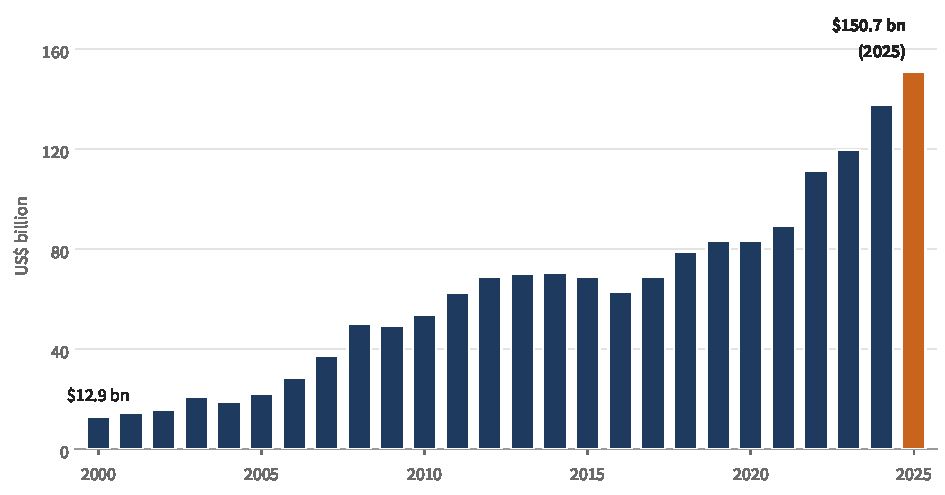
\includegraphics[width=\linewidth]{figures/remittances.pdf}
\captionof{figure}{Remittances received by India, 2000--2025 (US\$ billion).}\label{fig:m1-remit}
\figsource{World Bank (2026), World Development Indicators, series BX.TRF.PWKR.CD.DT.}
\raggedright
In 2025, Indians working abroad sent home \textbf{US\$150.7 billion}, more than any other country received and more than twice as much as Mexico, the next-largest recipient (World Bank, 2026). Where the money comes from is changing. In 2020-21 the US sent 23.4 per cent of it and the UAE 18.0 per cent. By 2023-24 the US share had risen to 27.7 per cent, while the UAE's had barely moved, to 19.2 per cent. An RBI study links this to more skilled Indians working in advanced economies (Gajbhiye et al., 2025).\par
\textbf{Read the chart.} (a) Roughly how many times larger were remittances in 2025 than in 2000? (b) In which year did they fall most sharply, and what might explain it?
\answers{(a) About 12 times (150.7 ÷ 12.9 ≈ 11.7). (b) 2016, when they fell about 9 per cent. The World Bank linked the fall to low oil prices and government spending cuts in the Gulf countries, where many Indians work (World Bank, 2017).}
\end{economistsfacts}

\begin{exercise}{Dollars in or dollars out?}
For each transaction, decide whether it adds to India's \emph{demand} for dollars or to the \emph{supply} of dollars.
\begin{enumerate}[label=(\alph*), leftmargin=2em]
  \item Meera's father pays her first-year fees.
  \item Ravi sends 3,000 dirhams to his parents in Thanjavur.
  \item A shop in New York pays Selvi for 5,000 T-shirts.
  \item A Japanese carmaker builds a new factory in Tamil Nadu.
  \item An Indian oil company buys a shipload of crude oil.
  \item An American investor sells her Indian shares and takes the money home.
  \item A family from Germany spends a week on a Kerala houseboat.
\end{enumerate}
\answers{Supply: (b), (c), (d), (g). Demand: (a), (e), (f).}
\end{exercise}

\begin{didyouknow}{Watch and learn}
Khan Academy's \emph{KA Macroeconomics Class 12} course, which follows the NCERT syllabus, has a short video on how currency exchange works: \href{https://www.khanacademy.org/economics-finance-domain/class-12-macroeconomics/x29cdf3f0a895464f:open-economy-macroeconomics/x29cdf3f0a895464f:foreign-exchange-market/v/currency-exchange-introduction}{\emph{Currency exchange introduction}}.
\end{didyouknow}

% ============================================================
%  SECTION A: The rupee's account book            (Member 1)
%  Defines "current account deficit" for Member 4 (Sections 7, D)
% ============================================================
\section*{A\quad The rupee's account book: the balance of payments}
\addcontentsline{toc}{section}{A\quad The rupee's account book: the balance of payments}

Every dollar that enters or leaves India is written down in the \keyterm{balance of payments (BoP)}{The record of all economic transactions between a country's residents and the rest of the world over a period.}, the record of all economic transactions between the residents of a country and the rest of the world over a period such as a year (NCERT, 2007). The \keyterm{current account}{The part of the BoP that records trade in goods and services, income and transfers.} records trade in goods and services, along with income and transfers such as remittances. The \keyterm{capital account}{The part of the BoP that records the buying and selling of assets, such as FDI, FPI and loans.} records the buying and selling of assets, such as FDI, FPI and foreign loans. When a country spends more foreign currency on its current account than it earns, it runs a \keyterm{current account deficit (CAD)}{The gap when a country's payments abroad for goods, services, income and transfers exceed its receipts.}. The gap must then be paid for by a net inflow on the capital account or by drawing down the country's reserves (NCERT, 2007).

India imports far more goods than it exports, mainly oil, gold and electronics. But software exports and remittances earn so much that they cover most of the gap. In 2025-26 these and other \keyterm{invisibles}{Trade in services, income and transfers, as opposed to trade in goods.} (services, income and transfers) brought in a net US\$312 billion, leaving a current account deficit of only US\$25.2 billion, about 0.6 per cent of GDP (RBI, 2026b). The capital account could not fill even this gap, because foreign portfolio investors took out a net US\$16.4 billion. So the RBI drew about US\$23.6 billion from its reserves \seesec{The RBI and India's foreign exchange reserves}.


% ---- Members 2, 3 and 4 insert their sections here ----
%  \input{sections/m2_sec3_demand_supply}
%  \input{sections/m2_sec4_appreciation}
%  \input{sections/m3_sec5_systems}
%  \input{sections/m3_sec6_real_ppp}
%  \input{sections/m4_sec7_what_moves}
%  \input{sections/m4_sec8_why_matters}

% ============================================================
%  CONCLUSION (end of chapter)                    (Member 1)
% ============================================================
\section*{Conclusion}
\addcontentsline{toc}{section}{Conclusion}

Now look again at Meera's fees. In 2026, dearer oil raised India's demand for dollars, while foreign investors selling Indian assets cut the supply \seesec{What moves the rupee?}. The RBI sold dollars from its reserves to slow the rupee's fall but did not stop it, and the bill for her fees went up by ₹2.5 lakh. The same move gave Ravi's family more rupees for every dirham. An exchange rate is just a price, but so much of India's trade, savings and borrowing passes through it that this one price reaches almost every household in the country.

% ============================================================
%  REFERENCES (Member 1 sections, APA 7th)
% ============================================================
\section*{References}
\addcontentsline{toc}{section}{References}
\begingroup\small\setlength{\parindent}{-1.5em}\setlength{\leftskip}{1.5em}\RaggedRight
Bank for International Settlements. (2025, September 30). \emph{Global FX trading hits \$9.6 trillion per day in April 2025 and OTC interest rate derivatives surge 79\%} [Press release]. \url{https://www.bis.org/media-releases/20250930-global-fx-trading-hits-96-trillion-day-april-2025-and-otc-interest-rate-derivatives-surge-79}\par\smallskip
Business Standard. (2025, October 13). \emph{Rupee recovers from day’s low even as oil prices advance, ends at 88.67/\$}. \url{https://www.business-standard.com/markets/news/rupee-recovers-from-days-low-even-as-oil-prices-advance-ends-at-88-67-per-dollar-125101300727_1.html}\par\smallskip
Chainwit. (2023). \emph{Arrival at Kathmandu Tribhuvan Airport (01-2023) - img 06} [Photograph]. Wikimedia Commons. CC BY 4.0. \url{https://commons.wikimedia.org/wiki/File:Arrival_at_Kathmandu_Tribhuvan_Airport_(01-2023)_-_img_06.jpg}\par\smallskip
Gajbhiye, D., Kundu, S., George, A., Vinherkar, O., Anees, Y., \& Baby, J. (2025, March 19). Changing dynamics of India’s remittances: Insights from the sixth round of India’s Remittances Survey. \emph{RBI Bulletin}. \url{https://www.rbi.org.in/Scripts/BS_ViewBulletin.aspx?Id=23260}\par\smallskip
Greenlaw, S. A., Shapiro, D., \& MacDonald, D. (2022). \emph{Principles of economics} (3rd ed.). OpenStax. \url{https://openstax.org/books/principles-economics-3e/pages/29-1-how-the-foreign-exchange-market-works}\par\smallskip
HDFC Sky. (2026, October 15). \emph{Rupee rises for 5th session, closes at 95.05 on RBI support}. \url{https://hdfcsky.com/news/inr-vs-usd-rate-october-15-2026}\par\smallskip
Jayadev, A. (2021). \emph{The economy: A South Asian perspective} (Version 1.0.1). CORE Econ. \url{https://books.core-econ.org/the-economy-south-asia/}\par\smallskip
Khan Academy. (n.d.). \emph{Currency exchange introduction} [Video]. KA Macroeconomics Class 12. \url{https://www.khanacademy.org/economics-finance-domain/class-12-macroeconomics/x29cdf3f0a895464f:open-economy-macroeconomics/x29cdf3f0a895464f:foreign-exchange-market/v/currency-exchange-introduction}\par\smallskip
Nagraj, A. (2024, November 22). Timeframe: When the UAE pegged its dirham to the US dollar in 1997. \emph{The National}. \url{https://www.thenationalnews.com/lifestyle/2024/11/22/uae-dirham-dollar-peg/}\par\smallskip
National Council of Educational Research and Training. (2007). \emph{Introductory macroeconomics: Textbook in economics for Class XII}. NCERT. \url{https://ncert.nic.in/textbook/pdf/leec106.pdf}\par\smallskip
Reserve Bank of India. (2022, July 11). \emph{International trade settlement in Indian rupees (INR)} (A.P. (DIR Series) Circular No. 10). \url{https://rbi.org.in/Scripts/NotificationUser.aspx?Id=12358}\par\smallskip
Reserve Bank of India. (2026a, January 21). Invoicing in INR of exports of goods and software and imports of goods. \emph{RBI Bulletin}, Table 39(a). \url{https://www.rbi.org.in/Scripts/BS_ViewBulletin.aspx?Id=23953}\par\smallskip
Reserve Bank of India. (2026b, June 8). \emph{Developments in India’s balance of payments during the fourth quarter (January–March) of 2025-26} [Press release]. \url{https://www.rbi.org.in}\par\smallskip
United Nations Conference on Trade and Development. (2025, March 14). \emph{Global trade update (March 2025)}. \url{https://unctad.org/news/global-trade-hits-record-33-trillion-2024-driven-services-and-developed-economies}\par\smallskip
World Bank. (2017, April 21). \emph{Remittances to developing countries decline for second consecutive year} [Press release]. \url{https://www.worldbank.org/en/news/press-release/2017/04/21/remittances-to-developing-countries-decline-for-second-consecutive-year}\par\smallskip
World Bank. (2026). \emph{Personal remittances, received (current US\$)} [Data set]. World Development Indicators. Retrieved October 16, 2026, from \url{https://data.worldbank.org/indicator/BX.TRF.PWKR.CD.DT}\par\smallskip
\endgroup


\end{document}
